%!TEX root = main.tex

\chapter{Basic Syntax and Semantics}

We are now ready to discuss the predicate logic, mostly the first-order logic. The language of predicate logic is more expressive than the one of propositional logic and allows us to express complex formulas in a much more concise way. In propositional logic, we often needed to use many variables and created long formulas. In predicate logic, some of these can be written more elegantly, as we can now use functions, relations, and logical quantifiers.

This whole part will follow the structure of the previous one -- we will again start by the basic syntax and semantics of predicate logic, then we will discuss the logical theories and their models, the tableau method in predicate logic and also the resolution method. While the basic ideas remain the same, there are also important differences. For example, a model of a theory will now be defined as a mathematical structure in which all the axioms of the theory are true, instead of the simpler definition as a truth assignment.

\section{First-order formulas and theories}

The symbols used in first-order language can be divided into two groups -- symbols of logic and non-logical symbols. The \emph{symbols of logic} consist of \emph{variables} ($x, y, z, \dots, x_1, x_2, \dots \in \SVar$), logical connectives $(\to, \land, \lor, \lequiv, \neg)$, the quantifiers $(\forall x), (\exists x)$ for each variable $x \in \SVar$, and parenthesis. 

The \emph{non-logical symbols} consist of function symbols $(f, g, \dots)$, including constant symbols ($c, d, \dots$), which are nullary function symbols, and relation (predicate) symbols $(P, Q, R)$. Each function and relation symbol $S$, has an associated arity $\ar(S)\in\Nat$ that expresses the number of arguments the symbol takes. 

The equality ($=$) is a special relation symbol that is often considered separately, as it is central to many parts of mathematics and there are even special axioms regarding the equality. Equality is also not considered a non-logical symbol.

The language in first-order logic is determined by the sets of function and relation symbols -- these are coupled in the so called \emph{signature}, which is a pair $\langle \mathcal{R}, \mathcal{F} \rangle$ of relation and function symbols with their arities. None of the symbols is the equality symbol. The \emph{language} is then given by a signature $L = \langle \mathcal{R}, \mathcal{F} \rangle$ and by specifying whether the language is with equality or not. A language must always contain at least one relation symbol (either equality or a non-logical one), otherwise, it would not be possible to write formulas in the language.

The meaning of the symbols in the language is not given by logic, i.e. even the common symbols like $+$ or $\leq$ do not need to represent addition or ordering.

There are many languages that are commonly used in mathematics, for example (all the languages are with equality):
\begin{enumerate}
  \item $L = \struct{ }$ is the language of pure equality,
  \item $L = \struct{c_i}_{i \in \Nat}$ is the language of countably many constants,
  \item $L = \struct{\leq}$ is the language of orderings,
  \item $L = \struct{E }$ is the language of graph theory,
  \item $L = \struct{+, -, 0}$ it the language of group theory,
  \item $L = \struct{+, -, \cdot, 0, 1}$ it the language of field theory,
  \item $L = \struct{-, \land, \lor, 0, 1}$ is the language of Boolean algebras, and
  \item $L = \struct{S, +, \cdot, 0, \leq}$ is the language of arithmetic.
\end{enumerate}
In the examples, $0$, $1$, and $c_i$ are constant symbols, $-$ and $S$ are unary function symbols, $+, \cdot, \land, \lor$ are binary function symbols, and $E$ and $\leq$ are binary relation symbols.

The structure of formulas in first-order language is more complex that the structure of propositional formulas. Before we formally define the formula, we first need to define terms and atomic formulas. Informally, terms are expressions created from variables and functions, while atomic formulas are relations applied to terms.

More formally, a \emph{term of a language $L$} is defined inductively as 
\begin{enumerate}
  \item Every variable $x \in \SVar$ or a constant symbol in $L$ is a term.
  \item If $f$ is a function symbol in $L$ with arity $n>0$ and $t_1, \dots, t_n$ are terms, then $f(t_1, \dots, t_n)$ is a term.
  \item Every term is obtained by finite amount of applications of steps 1 and 2 above.
\end{enumerate}

A term without variables is called a \emph{ground term}, the set of all terms of a language $L$ is denoted as $\Term_L$. A term that is a part of another term $t$ is called a \emph{subterm} of $t$. The terms can also be expressed using formation trees. For binary functions, we often use the infix notation, so we write $x+y$ instead of $+(x,y)$.

\begin{marginfigure}[-6\baselineskip]
\centering
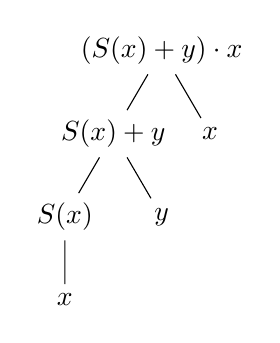
\begin{tikzpicture}[sibling distance=3.5em, level distance=3em]
  \node {$(S(x) + y)\cdot x$}
    child { node {$S(x)+y$} 
      child {node {$S(x)$}
      		child {node {$x$}}
      	}
      child {node {$y$}} }
    child { node {$x$} };
\end{tikzpicture}
\caption{A formation tree of the term $(S(x) + y)\cdot x$.}
\end{marginfigure}

The simplest type of formulas are the atomic formulas. These are only relations applied to terms. More formally, and \emph{atomic formula of a language $L$} is an expression $R(t_1, \dots, t_n)$, where $R$ is a relation symbol in $L$ and $t_1, \dots, t_n$ are terms of $L$. The set of all atomic formulas of language $L$ is denoted as $\AFm_L$. Similarly to terms, atomic formulas can also be represented using formation trees from the formation trees of its terms and for binary relations, we use the infix notation, e.g. $\leq(x, y)$ can be written as $(x \leq y)$. For example $(x + y) = 0$, or $R(f(x), g(y,z), x)$ are atomic formulas ($f$ is a unary function, $g$ and $+$ are binary functions, and $R$ is a ternary relation).

We can finally define formulas in first-order language. The definition is similar to the one in propositional language, but this time the propositional variables are represented by atomic formulas and we additionally have the quantifiers. Formally, a \emph{formula of a language $L$} is defined inductively by
\begin{enumerate}
  \item Every atomic formula is a formula
  \item If $\varphi$ and $\psi$ are formulas, $(\varphi \to \psi), (\varphi \land \psi), (\varphi \lor \psi), (\varphi \lequiv \psi), (\neg \varphi)$ are also formulas.
  \item If $\varphi$ is a formula and $x \in \SVar$ is a variable, then $((\forall x)\varphi)$ and $((\exists x)\varphi)$ are formulas.
  \item Every formulas is obtained by a finite application of the steps above.
\end{enumerate}

The set of all formulas of a language $L$ is denoted by $\Fm_L$. A formula that is a part of another formula $\varphi$ is a subformula of $\varphi$. Of course, formulas can also be expressed as their formation tree. An example is on the right.

\begin{marginfigure}[-6\baselineskip]
\centering
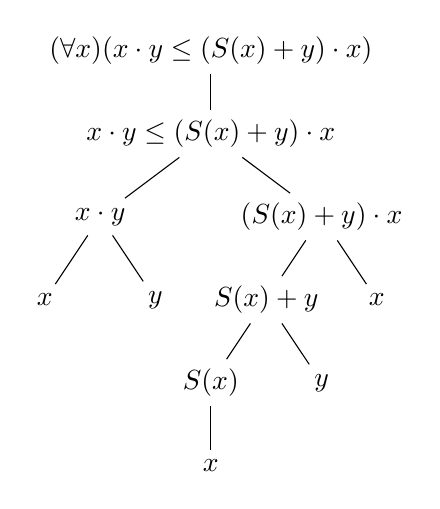
\begin{tikzpicture}[level 2/.style={sibling distance=8em}, 
                    level 3/.style={sibling distance=4em}, 
                    level distance=3em]
  \node {$(\forall x) (x \cdot y \leq (S(x) + y)\cdot x)$}
  	child {node {$x \cdot y \leq (S(x) + y)\cdot x$}
  		child {node {$x \cdot y$}
  			child {node {$x$}}
  			child {node {$y$}}
  		}
  		child {node {$(S(x) + y)\cdot x$}
  			child { node {$S(x)+y$} 
      		child {node {$S(x)$}
      			child {node {$x$}}
      		}
      	child {node {$y$}} 
      	}
      	child {node {$x$}}
      }
    };
\end{tikzpicture}
\caption{A formation tree of the formula $(\forall x) (x \cdot y \leq (S(x) + y)\cdot x)$. Moreover, $x\cdot y$ and $(S(x) + y)\cdot x$ are roots of formation trees of the terms included in the formula.}
\end{marginfigure}

As before, we can define some conventions to simplify writing the formulas. After introducing priorities of binary function symbols ($+, \cdot, \dots$) we can omit parenthesis in the infix notation of terms that are around a subterm formed by a symbol of higher priority. We also introduce the priority of logical connectives similar to the priorities in the propositional logic. The negation and quantifiers ($\neg, (\forall x), (\exists x)$) have the highest priorities, then we have conjunction and disjunction ($\land, \lor$) and, finally, the implication and equivalence ($\to, \lequiv$) have the lowest priority. Now, we can omit some of the parenthesis in the formulas.

In predicate logic, there is an important difference between so called free and bound (occurrences of) variables, as we deal with each type differently in the semantics. For a formula $\varphi$ and variable $x$, an \emph{occurrence of $x$ in $\varphi$} is a leaf labeled by $x$ in the formation tree of $\varphi$. The occurrence of $x$ in $\varphi$ is \emph{bound}, if it is in some subformula $\psi$ that starts with $(\forall x)$ or $(\exists x)$. Otherwise the occurrence is \emph{free}. A \emph{variable is free} in a formula, if it has at least one free occurrence in the formula and it is \emph{bound} if it has at least one bound occurrence. A variable can be both free and bound at the same time. For example, in formula $x > 0 \lor (\forall x) (\exists y)(x > y)$ the variable $x$ is both free and bound, as its first occurrence is free and the second one is bound. We will use the notation $\varphi(x_1, \dots, x_n)$ to denote that $x_1, \dots, x_n$ are all the free variables in $\varphi$.

A formula is \emph{open}, if it contains no quantifiers. The set of all open formulas in a language $L$ will be denoted as $\OFm_L$. Obviously, $\AFm_L \subsetneq \OFm_L \subsetneq \Fm_L$. On the other hand, a formula is \emph{closed (a sentence)} if it has no free variables. A formula can be both closed and open at the same time, all terms of such formulas are ground terms.

In mathematics, we very often have general theorems and we later use them with a more specific substitutions. This can more formally be expressed by substituting terms for free variables in formulas, however, we need to be careful, as in some cases the substitution can change the meaning of the formula. For example, if we substituted the term $y$ for $x$ in $(\exists y) (x+y=1)$, we would change the original meaning of the formula ``there is a $y$ such that $y = 1-x$'' to a new meaning that says ``y is divisible by 2''. We want to avoid such situation while performing the substitution. Therefore, we define a term $t$ is \emph{substitutable} for a variable $x$ in formula $\varphi$, if after the substitution of $t$ for all free occurrences of $x$, none of the variables of $t$ become bound in $\varphi$. The new formula is denoted as $\varphi(x/t)$ and we call it an \emph{instance of the formula $\varphi$} after a substitution of term $t$ for variable $x$. Alternatively, we can also define that $t$ is not substitutable for $x$ in $\varphi$ if $x$ has a free occurrence is a subformula of form $(\exists y)\psi$ or $(\forall y) \psi$ for some variable $y$ in $t$.

We can also rename the quantified variables, but we again need to be careful. In this case, we would like to obtain an equivalent formula. Let $(Qx)\psi$ us a subformula of $\varphi$ where $Q$ is either $\forall$ or $\exists$ and $y$ is a variable. Then, if $y$ is substitutable for $x$ in $\psi$ and $y$ is not free in $\psi$, we can replace the subformula $(Qx)\psi$ with $(Qy)\psi(x/y)$ to obtain a \emph{variant} of $\varphi$ in subformula $(Qx)\psi$. A variant of $\varphi$ is obtained by variation of one of more subformulas of $\varphi$.

\informal{Creating variants in predicate logic serves some important purposes. One of them is, that we can easily transform any formula with a variable that is both free and bound into its variant, where each variable is ``pure'', i.e. only free or only bound. Moreover, we will very often create variants from formulas in order to fulfill assumptions such as ``variable $x$ is not free in $\varphi$''.}

In propositional logic, models were defined as truth assignments. The truth assignment was enough to tell whether a proposition is true or false. In predicate logic, the situation is a bit more complex. First of all, the values of variables can be taken from a larger set than only $\{0,1\}$. Moreover, we need to define, what all the functions a relations mean. A natural representation of models in first-order logic is a mathematical structure. A structure is a set and a definition of functions and relations on this set. 

More formally, if we have a signature of a language $L = \langle \mathcal{R}, \mathcal{F} \rangle$ and a non-empty set $A$. A \emph{realization (interpretation) of a relation symbol} $R \in \mathcal{R}$ on set $A$ is any relation $R^A \subseteq A^{\ar(R)}$. A realization of $=$ is the identity relation on $A$, i.e. $\mathrm{Id}_A = \{(x, x) | x \in A\}$. \emph{A realization (interpretation) of a function symbol} $f \in \mathcal{F}$ is any function $f^A: A^{\ar(f)} \to A$. Specifically, a realization of a constant symbol is some element of $A$. A \emph{structure for the language $L$} ($L$-structure) is a triple $\mathcal{A} = \langle A, \mathcal{R}^A, \mathcal{F}^A \rangle$, where $A$ is a non-empty set called the domain of the structure $\mathcal{A}$, $\mathcal{R}^A$ is a collection of realizations of the relation symbols on $A$, and $\mathcal{F}^A$ is a collection of realizations of function symbols on $A$. A structure of the language is also called a model of the language, and the class of all models of a language $L$ will be denoted as $M(L)$.

You probably already know different mathematical structures from other parts of mathematics, for example:
\begin{enumerate}
	\item $S = \struct{S, \leq}$ is an ordered set, where $\leq$ is reflexive, antisymmetric, and transitive binary relation,
	\item $G = \struct{V, E}$ is a graph,
	\item $\Int_p = \struct{\Int_p, +, -, 0}$ is the additive group of integers modulo $p$,
	\item $\Rat = \struct{\Rat, +, -, 0, 1}$ is the field of rational numbers,
	\item $\mathcal{P}(X) = \struct{\mathcal{P}(X), \setminus, \cap, \cup, \emptyset, X}$ is the set algebra over $X$, and
	\item $\Nat = \struct{\Nat, S, +, \cdot, 0, \leq}$ is the standard model of arithmetic.
\end{enumerate}
But also many other objects can be defined as structures, e.g. the finite automata or even databases.

We now aim to define the truth value of formulas in first-order logic. We already know, that a formula is constructed from atomic formulas, which are in turn constructed from terms. Therefore, in order to define the truth value of a formula, we need to start with the definition of the value of a term. Let $t$ be a term of $L = \struct{\cR, \cF}$ and $\cA = \struct{A, \cR^A, \cF^A}$ an $L$-structure. A \emph{variable assignment} over the domain $A$ is a function $e: \SVar \to A$. The \emph{value $t^A[e]$ of term $t$} in structure $\cA$ with respect to the assignment $e$ is defined inductively by 
\begin{enumerate}
	\item $x^A[e] = e(x)$, for $x \in \SVar$,
	\item $(f(t_1, \dots, t_n))^A[e] = f^A(t_1^A[e], \dots, t_n^A[e])$ for $f \in \cF$.
\end{enumerate}
For a constant symbol $c^A[e] = c^A$, i.e. the values of constants do not depend on the assignment $e$, and therefore also the value of ground terms does not depend on the assignment. Obviously, the value of a term $t$ depends only on the assignment of variables in $t$.

We now know, how to compute the values of individual terms, therefore, we can define the value of atomic formulas. Contrary to the values of terms, values of formulas are always from the set $\{0,1\}$. Let $\varphi$ be an atomic formula of $L = \struct{\cR, \cF}$ in the from $R(t_1, \dots, t_n)$, $\cA = \struct{A, \cR^A, \cF^A}$ is an $L$-structure and $e$ a variable assignment over $A$. The \emph{value $H^A_{at}(\varphi)[e]$ of the atomic formula $\varphi$} in the structure $A$ with respect to $e$ is $$H^A_{at}(\varphi)[e] = \twopartdefotherwise{1}{(t_1^A[e], \dots t_n^A[e]) \in R^A}{0}$$

Specifically, for the equality relation $=$, the only possible realization is $\mathrm{Id}_A$ and therefore $H^A_{at}(t_1=t_2)[e] = 1$, if $t_1^A[e]=t_2^A[e]$ and $0$ otherwise. We can again see that the value of a formula depends only on the assignment of variables in the formula and that the value of a ground formula does not depend on the assignment at all.

We can finally define the value of a general formula. The definition is quite long, but also very similar to the one in propositional logic. In fact, the only difference is in the last two cases. The atomic formulas in this case play the role of the propositional variables.

The value $H^A(\varphi)[e]$ of formula $\varphi$ in the structure $A$ with respect to $e$ is 
\begin{enumerate}
	\item $H^A(\varphi)[e] = H^A_{at}(\varphi)[e]$ if $\varphi$ is atomic
	\item $H^A(\neg \varphi)[e] = -_1(H^A(\varphi)[e])$
	\item $H^A(\varphi \land \psi)[e] = \land_1(H^A(\varphi)[e], H^A(\psi)[e])$
	\item $H^A(\varphi \lor \psi)[e] = \lor_1(H^A(\varphi)[e], H^A(\psi)[e])$
	\item $H^A(\varphi \to \psi)[e] = \to_1(H^A(\varphi)[e], H^A(\psi)[e])$
	\item $H^A(\varphi \lequiv \psi)[e] = \lequiv_1(H^A(\varphi)[e], H^A(\psi)[e])$
	\item $H^A((\forall x)\varphi)[e] = \min_{a \in A}(H^A(\varphi)[e(x/a)])$
	\item $H^A((\exists x)\varphi)[e] = \max_{a \in A}(H^A(\varphi)[e(x/a)])$
\end{enumerate}
where $-_1, \land_1, \lor_1, \to_1, \lequiv_1$ are the function given by the truth tables in the part on propositional logic and $e(x/a)$ is an assignment  assigning value $a$ to variable $x$ and otherwise identical to $e$. We can see that the value of a formula depends only on the assignment of free variables in the formula (we check all possible assignments for the bound variables in steps 7 and 8).

The structure $\cA$ satistifies the formula $\varphi$ if $H^A(\varphi) = 1$, we denote the fact as $\cA \vDash \varphi[e]$, otherwise we write $\cA \nvDash \varphi[e]$. We can easily check that all the following hold
\begin{align*}
\cA \vDash \neg \varphi[e] & \Leftrightarrow \cA \nvDash \varphi[e] \\
\cA \vDash (\varphi \land \psi)[e] & \Leftrightarrow \cA \vDash \varphi[e] \text{ and } \cA \vDash \psi[e]\\
\cA \vDash (\varphi \lor \psi)[e] & \Leftrightarrow \cA \vDash \varphi[e] \text{ or } \cA \vDash \psi[e]\\ 
\cA \vDash (\varphi \to \psi)[e] & \Leftrightarrow \cA \vDash \varphi[e] \text{ implies } \cA \vDash \psi[e]\\
\cA \vDash (\varphi \lequiv \psi)[e] & \Leftrightarrow \cA \vDash \varphi[e] \text{ if and only if } \cA \vDash \psi[e]\\
\cA \vDash (\forall x)(\varphi)[e] & \Leftrightarrow \cA \vDash \varphi[e(x/a)] \text{ for every } a \in A \\
\cA \vDash (\exists x)(\varphi)[e] & \Leftrightarrow \cA \vDash \varphi[e(x/a)] \text{ for some } a \in A
\end{align*}
Furthermore, if $t$ is substitutable for $x$ in $\varphi$, then for every structure $\cA$ and assignment $e$, $\cA \vDash \varphi(x/t)[e]$ if and only if $\cA \vDash \varphi[e(x/a)]$, where $a = t^A[e]$. If $\psi$ is a variant of $\varphi$ then $\cA \vDash \varphi[e]$ if and only if $\cA \vDash \psi[e]$.

As in propositional logic, we can generalize the notion above to validity in structure and in theory. Let $\varphi$ be a formula of a language $L$, and $\cA$ an $L$-structure. We say, that \emph{$\varphi$ is valid in $\cA$}, denoted as $\cA \vDash \varphi$, if $\cA \vDash \varphi[e]$ for every $e: \SVar \to A$. We also say that \emph{$\cA$ satisfies $\varphi$}. Otherwise, we write $\cA \nvDash \varphi$. The formula \emph{$\varphi$ is contradictory in $\cA$} if $\cA \vDash \neg \varphi$, i.e. if $\cA \nvDash \varphi[e]$ for every $e$.

We can easily check, that for any structure $\cA$ and formulas $\varphi, \psi$ the following holds:
\begin{align}
	\cA \vDash \varphi & \Rightarrow \cA \nvDash \neg \varphi \\
	\cA \vDash \varphi \land \psi & \Leftrightarrow \cA \vDash \varphi \text{ and } \cA \vDash \psi\\
	\cA \vDash \varphi \lor \psi & \Leftarrow \cA \vDash \varphi \text{ or } \cA \vDash \psi\\
	\cA \vDash \varphi & \Leftrightarrow \cA \vDash (\forall x)\varphi
\end{align}
Moreover, if $\varphi$ and $\psi$ are sentences, the implications in (1) and (3) are in fact equivalences. The last equivalence (4) also shows, that $\cA \vDash \varphi$ if and only if $\cA \vDash \psi$, where $\psi$ is the \emph{universal closure} of $\varphi$, i.e. the formula $(\forall x_1)(\forall x_1) \dots (\forall x_n)\varphi$, where $x_1, \dots, x_n$ are all the free variables of $\varphi$.

A \emph{theory} of a language $L$ is any set $T$ of formulas of $L$ (the \emph{axioms} of the theory). A \emph{model of a theory $T$} is an $L$-structure $\cA$ such that $\cA \vDash \varphi$ for every $\varphi \in T$. We also write $\cA \vDash T$ and say that $\cA$ satisfies $T$. The \emph{class of all models} of theory $T$ is $M(T) = \{\cA \in M(L) | \cA \vDash T\}$. A formula is \emph{valid in $T$} (true in $T$) ($T\vDash \varphi$) if $\cA \vDash \varphi$ for every model $\cA$ of $T$. Otherwise we write $T \nvDash \varphi$. A formula \emph{$\varphi$ is contradictory in $T$} if $T \vDash \neg \varphi$ and \emph{$\varphi$ is independent in $T$} if it is neither valid nor contradictory in $T$. For empty theory $T$, we can omit $T$ in the notation and $M(T)=M(L)$. In this case, ($\vDash T$) means that the formula $\varphi$ is \emph{logically valid} (\emph{a tautology}). A \emph{consequence of $T$} is the set $\theta^L(T)$ of all sentences of $L$ valid in $T$, i.e. $$\theta^L(T) = \{\varphi \in \Fm_L\ | T\vDash \varphi \text{ and } \varphi \text{ is a sentence}\}\,.$$

\informal{The definitions above should closely resemble those we saw in propositional logic, the main difference is in the definition of the model. In propositional logic, we could use truth assignments, while in predicate logic, the model is a structure. The structure, and its definitions of functions and relations in fact give the truth values to the atomic formulas. The atomic formulas than play the role of the propositional variables. Of course, in predicate logic, we also need to take care of the quantifiers, which brings another complexity to the definitions.}